% !TEX root = ../main.tex
\chapter{Combining Sentiment Analysis and Topic Modeling}
\label{ch:combiningSentimentAnalysisAndTopicModeling}

% TODO write about "Joint sentiment/topic model for sentiment analysis" here and/or in the related-work section

In this chapter, the best sentiment analysis model from~\cref{ch:sentimentAnalysis}, naive Bayes,
is combined with the LDA topic model built in~\cref{ch:topicModeling},
to perform the sentiment analysis by topic referred to in~\cref{sec:backgroundTheory}.
\\
This is achieved by simply performing the sentiment analysis on a Twitter status and attributing the result to each topic,
weighed by the percentage the status belongs to that topic given by the topic model.
A pseudo-code implementation of that can be seen in~\cref{pseudo_code:sentiment_topic_summing}.

\begin{figure}
    \caption{Summing up sentiments by topic for each status}
    \label{pseudo_code:sentiment_topic_summing}
    % @formatter:off
    \begin{algorithmic}
        \State $topic\_sentiments \gets {}$ %
        \For{$status$ in $statuses$}
            \State $topic\_probabilities \gets LDA(status)$
            \State $sentiment \gets naive_bayes(status)$
            \For{$topic,probability$ in $topic\_probabilities$}
                \State $topic\_sentiments[topic][sentiment]
                    \gets topic\_sentiments[topic][sentiment] + probability$
            \EndFor
        \EndFor
    \end{algorithmic}
    % @formatter:on
\end{figure}

This results in a 2-dimensional array where all values sum up to the number of statuses,
since for each status the topic-probabilities sum up to 1.
This was then performed on the sample stream dataset collected in~\cref{sec:streamingSampleDataset}.
A table showing the results for each topic with relative as well as absolute values for the sentiment classes can be seen in~\cref{tab:combination}.
The table also shows the sum of all probabilities, and the percentage of statuses in that topic.

\begin{table}
    \caption{Absolute and relative results of the sentiment-by-topic analysis on the sample stream dataset}
    \label{tab:combination}
    \resizebox{\textwidth}{!}{%
    \begin{tabular}{l l l l l l l l l l l l} %
        \toprule
        & &
        \multicolumn{2}{c}{Positive}&
        \multicolumn{2}{c}{Neutral}&
        \multicolumn{2}{c}{Negative}&
        \multicolumn{2}{c}{Irrelevant}&
        \multicolumn{2}{c}{Sum}
        \\\cmidrule{3-12}
        Topic & Top 5 Terms
        & Abs.
        & \%
        & Abs.
        & \%
        & Abs.
        & \%
        & Abs.
        & \%
        & Abs.
        & \%
        \\\midrule
        0 & read, seo, old, board, actually & 64.40 & 11.14\% & 267.00 & 46.18\% & 56.67 & 9.80\% & 190.16 & 32.89\% & 578.23 & 9.00\% \\\midrule
        1 & time, single, playing, weekend, face & 74.44 & 11.43\% & 313.13 & 48.09\% & 92.87 & 14.26\% & 170.75 & 26.22\% & 651.19 & 10.14\% \\\midrule
        2 & need, give, damn, remember, already & 59.00 & 9.24\% & 302.46 & 47.39\% & 80.35 & 12.59\% & 196.43 & 30.78\% & 638.24 & 9.94\% \\\midrule
        3 & people, back, prove, sorry, tonight & 96.24 & 13.93\% & 320.69 & 46.40\% & 78.08 & 11.30\% & 196.10 & 28.37\% & 691.11 & 10.76\% \\\midrule
        4 & trump, enough, world, love, adamu & 69.94 & 11.08\% & 326.17 & 51.65\% & 79.75 & 12.63\% & 155.64 & 24.65\% & 631.50 & 9.83\% \\\midrule
        5 & home, people, morning, appears, shit & 82.30 & 12.48\% & 278.07 & 42.16\% & 94.26 & 14.29\% & 204.97 & 31.08\% & 659.59 & 10.27\% \\\midrule
        6 & love, win, chance, follow, enter & 63.83 & 10.96\% & 297.55 & 51.08\% & 53.85 & 9.24\% & 167.27 & 28.72\% & 582.51 & 9.07\% \\\midrule
        7 & mtvhottest, lady, gaga, larsson, zara & 42.43 & 7.65\% & 253.08 & 45.62\% & 43.23 & 7.79\% & 216.02 & 38.94\% & 554.75 & 8.64\% \\\midrule
        8 & miss, sexy, sex, naked, outfit & 79.47 & 11.54\% & 344.14 & 49.97\% & 63.95 & 9.29\% & 201.15 & 29.21\% & 688.71 & 10.72\% \\\midrule
        9 & tell, someone, feel, every, preaching & 74.32 & 10.80\% & 327.11 & 47.54\% & 94.52 & 13.74\% & 192.12 & 27.92\% & 688.05 & 10.71\%
        \\\bottomrule
    \end{tabular}}
\end{table}

To visualize the sentiment by topic,
the network graph used in~\cref{ch:topicModeling} was extended.
The size of a node representing a topic indicates the topics' prevalence in the dataset.
The color, on a hue-spectrum from red to green represents the polarity.
On a 360\degree hue-spectrum in the HSV-color-space, as seen in~\cref{fig:hue_spectrum}, 0\degree is red, and 120\degree is green.

\begin{figure}
    \centering
    \caption{Hue-spectrum~\cite{hueSpectrum}}
    \label{fig:hue_spectrum}
    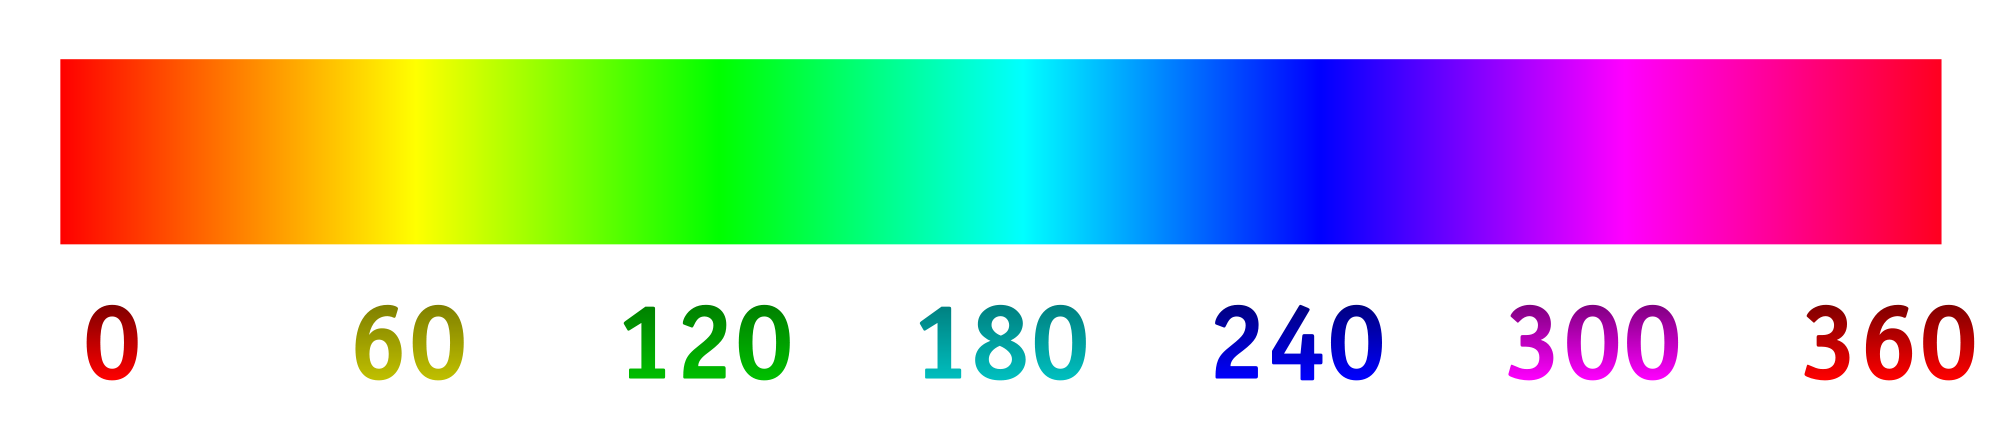
\includegraphics[width=10cm]{../images/hue_spectrum.png}
\end{figure}

The opacity is determined by the subjectivity.
The exact formulae can be seen in~\cref{math:visualization}.

\begin{figure}
    \caption{The formulae used to extend the network graph}
    \label{math:visualization}
    \begin{math}
        \\
        size = positive + negative + neutral + irrelevant\\
        hue = positive / (positive + negative)\\
        opacity = (positive + negative) / (positive + negative + neutral)\\
        prevalence = \textrm{percentage of statuses in that topic}\\
        size = prevalence \times 2000\\
    \end{math}
\end{figure}

To make these values visually more differentiable, they were then scaled.
Hue was linearly scaled such that the smallest value was 0\degree (red) and the biggest value was 120\degree (green).
The saturation was linearly scaled such that the smallest opacity was 0\%,
and the biggest opacity was 80\%.
20\% were then added to each node, making sure each node is visible.
The size was linearly scaled to be between 0 and 2000.
The resulting network graph can be seen in~\cref{fig:combined_network_graph}.

\begin{figure}
    \centering
    \caption{Network graph of the LDA topic model created from the stream sample dataset}
    \label{fig:combined_network_graph}
    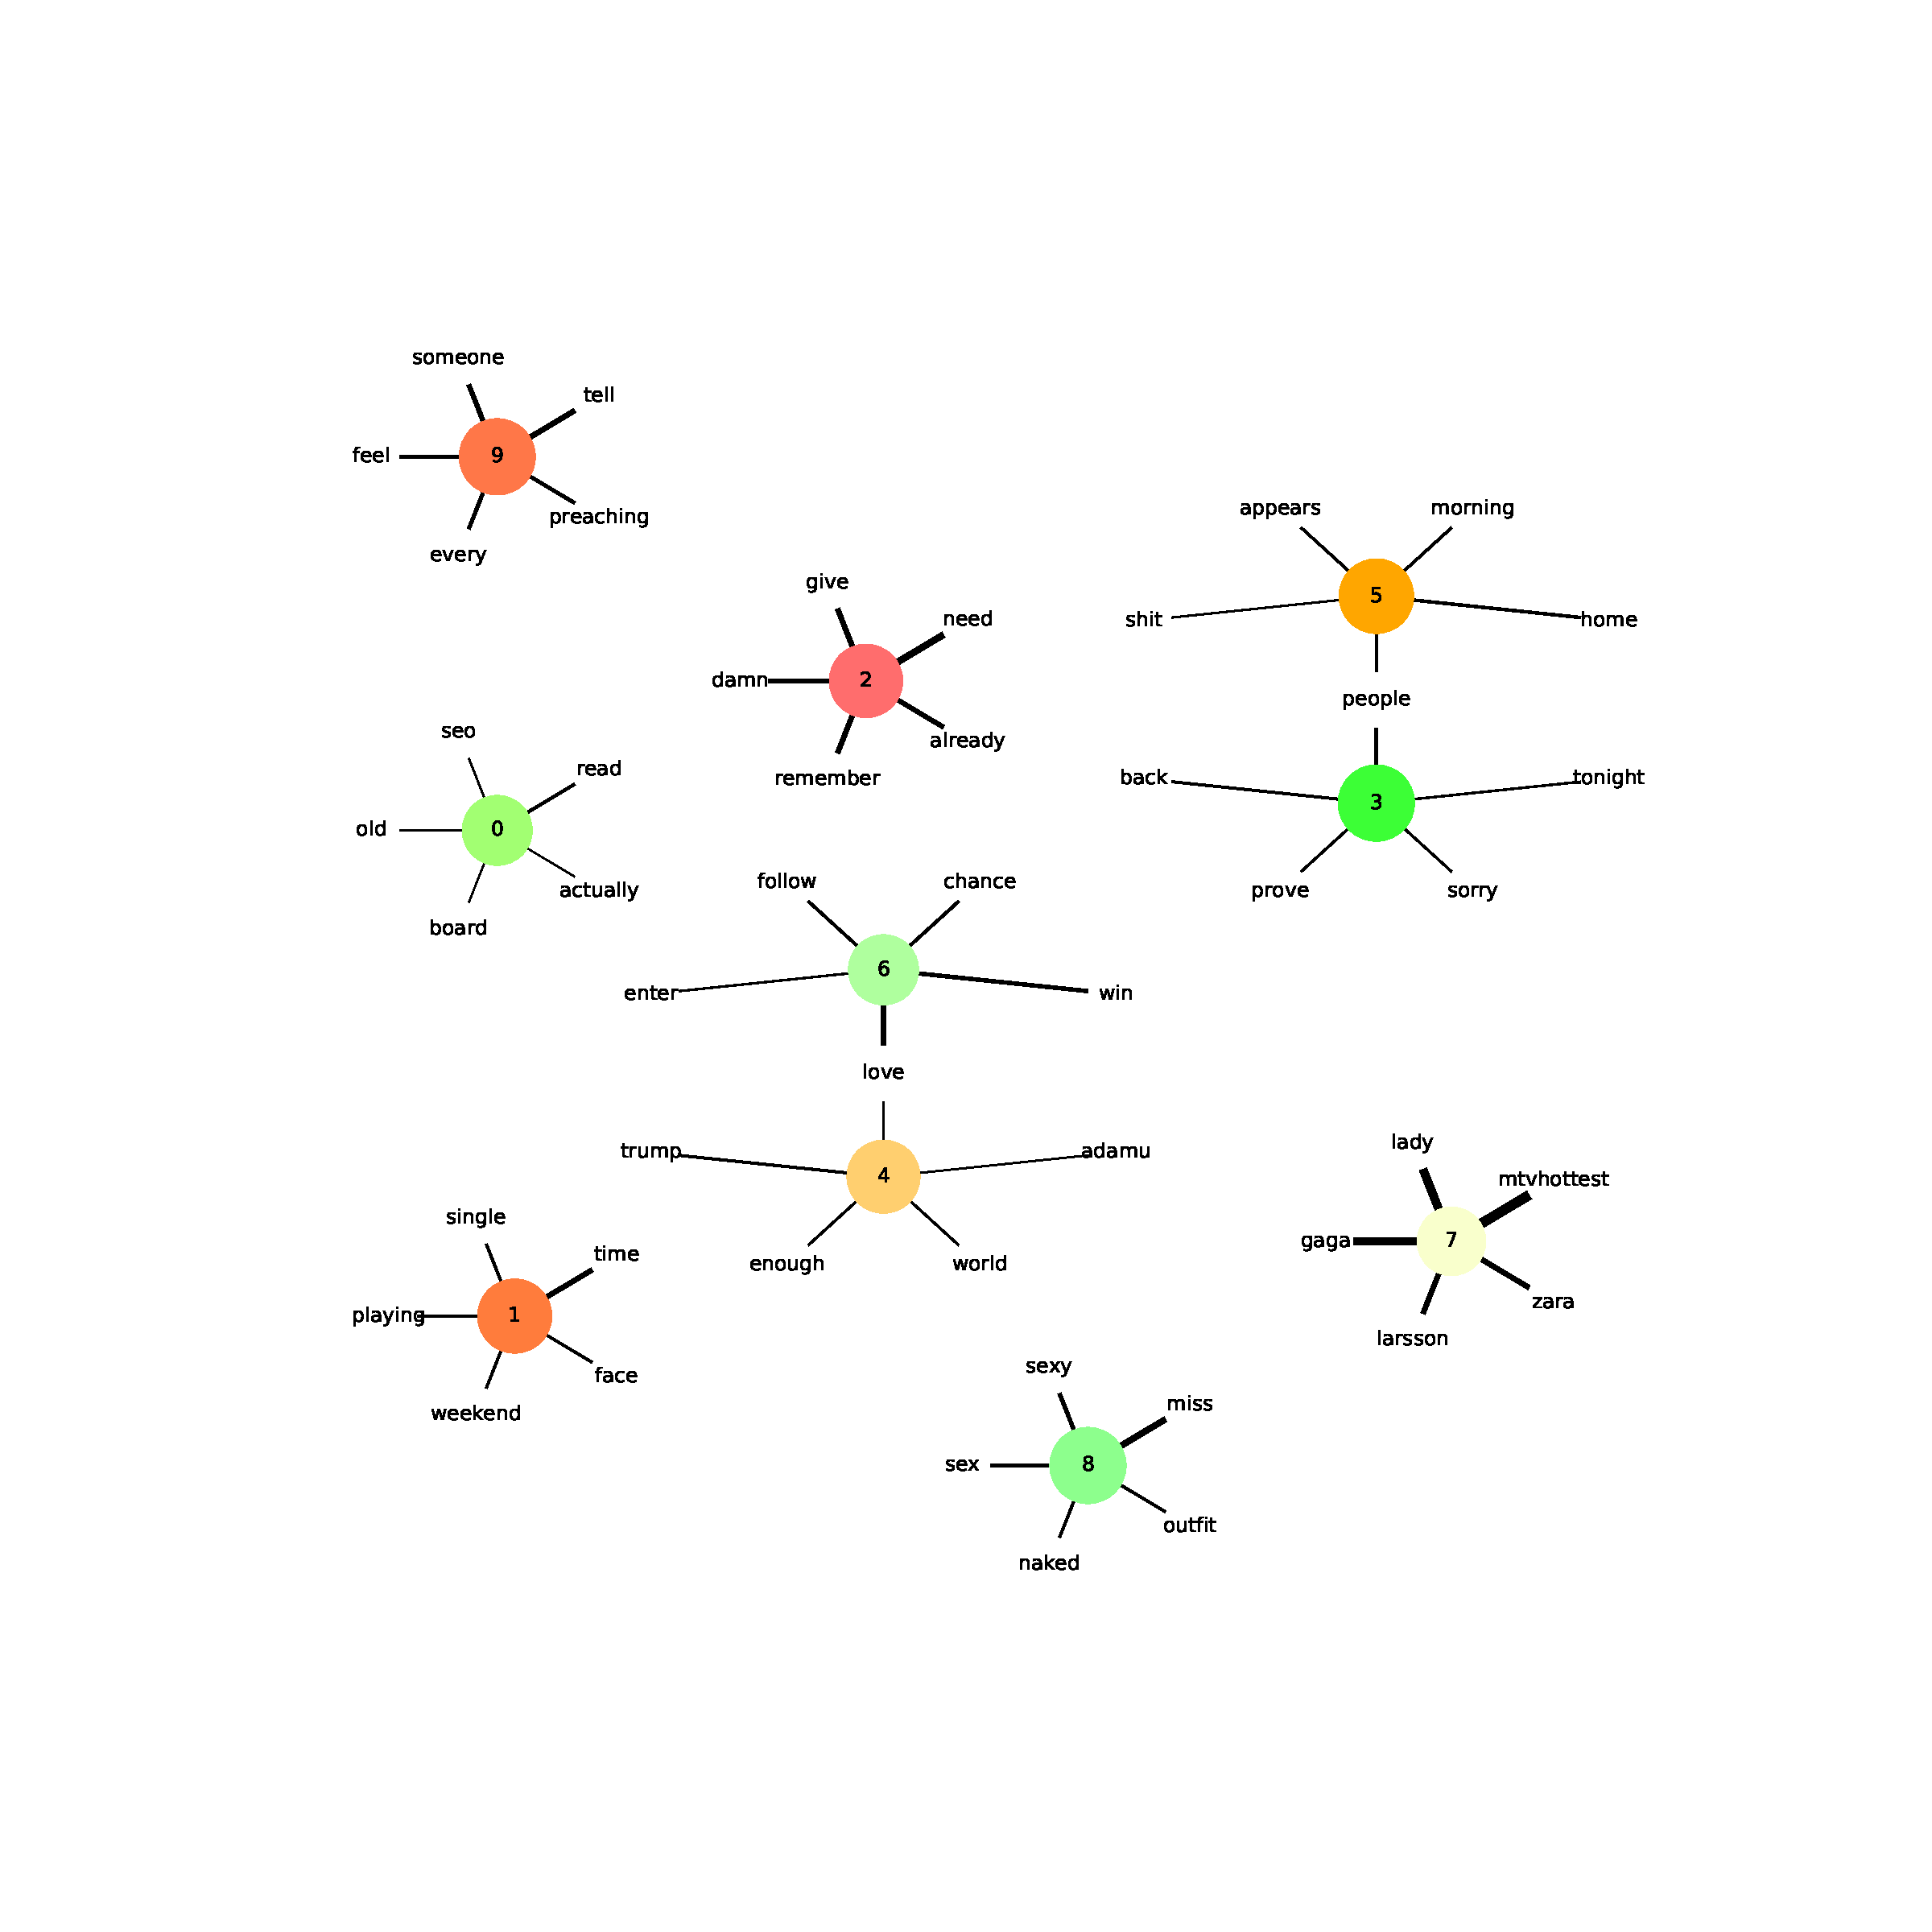
\includegraphics[width=\textwidth]{../figures/combined_network_graph.pdf}
\end{figure}